\documentclass{beamer}
\setbeamertemplate{background canvas}[vertical shading][bottom=red!10,top=blue!10]
\usetheme{Berkeley}
\usepackage[utf8]{vietnam}
\usepackage{tikz}
\usepackage{hyperref}
\usepackage{booktabs, multicol, multirow}
\usepackage{adjustbox}
\graphicspath{ {images/} }

\title{Luận văn tốt nghiệp}
\subtitle{Giải quyết đồng tham chiếu cho các đối tượng và thuộc tính trong khai khoáng ý kiến}
\author[]{Nguyễn Trọng Nghĩa 51202370 \\ Nguyễn Đăng Trang 51203957 \\ GVHD: GS. Phan Thị Tươi}
\institute{Đại học Bách Khoa TP. Hồ Chí Minh}
\date{\today}

\begin{document}

\setbeamertemplate{sidebar left}[sidebar theme]
\begin{frame}
\titlepage
\end{frame}

\section{Giới thiệu đề tài}
\begin{frame}
\frametitle{Giới thiệu đề tài}
\begin{block}{}
\textbf{Giải quyết đồng tham chiếu cho đối tượng và thuộc tính trong khai khoáng ý kiến} là một bài toán con của bài toán giải quyết đồng tham chiếu trong Xử lý ngôn ngữ tự nhiên (XLNNTN), với chủ thể hướng đến là các đối tượng và thuộc tính. Đối tượng và thuộc tính đều là các thực thể, trong đó thuộc tính là bộ phận hoặc đặc tính của đối tượng.
\end{block}
\begin{block}{}
Phân giải đồng tham chiếu trên các văn bản có chứa ý kiến của người dùng như các review, discussion, ... là một hướng đi mới so với phân giải đồng tham chiếu nói chung.
\end{block}
\end{frame}

\begin{frame}
\frametitle{Giới thiệu đề tài}
\begin{block}{}
Khai khoáng ý kiến (Opinion Mining) là một lĩnh vực mới được phát triển và ngày càng có nhiều ứng dụng trong nhiều lĩnh vực.
\end{block}
\begin{block}{}
Trong các văn bản có chứa ý kiến, nếu không có phân giải đồng tham chiếu cho các đối tượng và thuộc tính, ý kiến của người viết rất có thể sẽ được gán không đúng cho các thực thể.
\end{block}
\begin{block}{}
Các từ ngữ chỉ ý kiến (gắn với các thực thể) có thể được sử dụng là một phần trong các thuộc tính để giải quyết bài toán đồng tham chiếu (sẽ được trình bày ở các slide sau).
\end{block}
\end{frame}

\begin{frame}
\frametitle{Giới thiệu đề tài}
\begin{block}{}
Ví dụ 1: \\
I've had \textbf{\textcolor{red}{my 8100}} for about two years.  Dropped \textbf{\textcolor{red}{it}} on pavement, concrete, wood floors, etc. at least 30 times so \textbf{\textcolor{red}{it}} has a ton of scratches but \textbf{\textcolor{red}{it}}'s held up very well.  My 2-year old has chewed on \textbf{\textcolor{red}{it}}, licked \textbf{\textcolor{red}{it}}, smacked \textbf{\textcolor{red}{it}}, etc. -- still no problems.  \textbf{Signal} has been solid, \textbf{intuitive usability} is very good.  \textbf{My standard battery} was great for the first 20 months (several hours of \textbf{talk time}, a week of \textbf{standby}) and just now is needing a charge every other day. I'll definitely buy a Sanyo again.
\end{block}
\end{frame}

\begin{frame}
\frametitle{Giới thiệu đề tài}
\begin{block}{}
Trong review trên, đối tượng được nói đến là một chiếc điện thoại \textbf{my 8100}. Nó bao gồm các thuộc tính là \textbf{a ton of scratches}, \textbf{Signal}, \textbf{intuitive usability}, \textbf{My standard battery}, \textbf{talk time} và \textbf{standby}. Trên thực thể và các thuộc tính này, người dùng có thể hiện ý kiến cá nhân lên nó. Ví dụ: \textit{Signal has been solid}. 
\end{block}
\begin{block}{}
Các từ/cụm từ \textbf{my 8100} và \textbf{it} (được bôi đỏ) trong ví dụ trên đồng tham chiếu với nhau, nó cùng chỉ tới một thực thể là chiếc điện thoại \textbf{my 8100}.
\end{block}
\end{frame}

\section{Khái quát về đồng tham chiếu}
\begin{frame}
\frametitle{Giới thiệu bài toán giải quyết đồng tham chiếu trong Xử lý ngôn ngữ tự nhiên}
\begin{block}{}
\textbf{Phân giải đồng tham chiếu} là một bài toán kinh điển trong XLNNTN. Hai từ hoặc cụm từ được gọi là đồng tham chiếu với nhau nếu chúng cùng chỉ đến một thực thể.
Mục tiêu của bài toán phân giải đồng tham chiếu là tìm kiếm tất cả các từ hoặc cụm từ đồng tham chiếu với nhau đó.
\end{block}
\begin{block}{}
Có 3 hướng tiếp cận phổ biến đối với bài toán Phân giải đồng tham chiếu:
\begin{itemize}
\item Phương pháp học có giám sát
\item Phương pháp học không giám sát
\item Phương pháp xây dựng hệ thống các luật
\end{itemize}
\end{block}
\end{frame}
\begin{frame}
\frametitle{Các hướng tiếp cận giải quyết bài toán}
\begin{block}{}
\textbf{Phương pháp học có giám sát}
\begin{itemize}
\item Hai giải thuật được sử dụng phổ biến: Cây quyết định và SVM
\item Mô hình xây dựng tập huấn luyện: Mô hình xét theo cặp, mô hình hướng thực thể, mô hình xếp hạng.
\end{itemize}
\end{block}
\begin{block}{}
\textbf{Phương pháp học không giám sát:} Giải thuật thường được sử dụng là giải thuật gom cụm.
Mỗi từ, cụm từ có một tập các thuộc tính đặc trưng. Giải thuật gom cụm phân chia tập các từ, cụm từ thành các cụm, trong đó mỗi cụm chứa các từ, cụm từ có cùng đặc điểm về thuộc tính.
\end{block}
\end{frame}

\begin{frame}
\frametitle{Các hướng tiếp cận giải quyết bài toán}
\begin{block}{}
\textbf{Phương pháp xây dựng hệ thống các luật:} Xây dựng tập luật gồm các luật về cú pháp, ngữ nghĩa xác định khi nào thì hai từ, cụm từ đồng tham chiếu đến nhau. Luật đứng đầu tiên có độ chính xác cao nhất, sau đó giảm dần với các luật đứng sau. Văn bản được đưa qua các luật, bắt đầu từ luật đầu tiên. Sau khi áp dụng tất cả các luật trên văn bản, ta thu được kết quả cuối cùng là tập các cụm đồng tham chiếu.
\end{block}
\end{frame}

\section{Khái quát về khai khoáng ý kiến}
\begin{frame}
\frametitle{Giới thiệu về khai khoáng ý kiến}
\begin{block}{}
\textbf{Khai khoáng ý kiến (Opinion Mining)} hay \textbf{Phân tích cảm xúc (Sentiment Analysis)} là một lĩnh vực nghiên cứu của Xử lý ngôn ngữ tự nhiên (XLNNTN), hướng đến việc tìm ra ý kiến/cảm xúc của chủ thể (người viết, người nói,...) đối với một thực thể nào đó thể hiện qua ngôn ngữ.
\end{block}
\begin{block}{}
Các mô hình khai khoáng ý kiến:
\begin{itemize}
\item{Cấp độ văn bản (Document level)}
\item{Cấp độ câu (Sentence level)}
\item{Cấp độ thực thể - thuộc tính (Entity-Aspect level)}
\end{itemize}
\end{block}
\end{frame}

\begin{frame}
\frametitle{Khai khoáng ý kiến cấp độ thực thể - thuộc tính}
\begin{block}{}
Ở cấp độ thực thể - thuộc tính, nhiệm vụ là tìm tất cả các ý kiến (Opinion) chứa trong văn bản: Một ý kiến bao gồm 5 thành phần (Theo Bing Liu trong cuốn Sentiment Analysis and Opinion Mining \footnote{https://www.cs.uic.edu/~liub/FBS/SentimentAnalysis-and-OpinionMining.pdf})
\\\textbf{(e,a,s,h,t)}
\\\textbf{e}: thực thể
\textbf{a}: thuộc tính của thực thể
\textbf{s}: ý kiến trên thực thể đó
\textbf{h}: chủ thể thể hiện ý kiến
\textbf{t}: thời điểm đưa ra ý kiến
\end{block}
\begin{block}{}
Ví dụ: Một ý kiến được rút trích từ \textit{ví dụ 1} \{my 8100, my battery, tích cực (great), người viết review, thời gian viết review\}
\end{block}
\end{frame}

\section{Phương pháp đề xuất}
\begin{frame}
\frametitle{Phương pháp đề xuất}
% Author: Rasmus Pank Roulund
%\documentclass{minimal}
%\usepackage{tikz}
%\usepackage[utf8]{vietnam}

%\begin{document}
\usetikzlibrary{arrows,chains,positioning,scopes}

\tikzset{
    block/.style={draw,text width=4em,minimum height=6.5em,minimum width=4em,align=center},
    arrow/.style={->, thick}
}
\begin{tikzpicture}
  {[start chain]
        \node[block,on chain] (N1) {Thu thập dữ liệu thô};
        \node[block,on chain,join=by {arrow},right=0.7cm of N1] (N2) {Tiền xử lý dữ liệu};
        \node[block,on chain,join=by {arrow},right=0.7cm of N2] (N3) {Trích xuất cụm danh từ};
        \node[block,on chain,join=by {arrow},right=0.7cm of N3] (N4) {Gán nhãn dữ liệu};
       \node[block,on chain,join=by {arrow},below=0.7cm of N4] (N5) {Trích xuất thuộc tính};
       \node[block,on chain,join=by {arrow},left=0.7cm of N5] (N6) {Tạo tập huấn luyện và tập kiểm tra};
       \node[block,on chain,join=by {arrow},left=0.7cm of N6] (N7) {Áp dụng giải thuật học máy};
       \node[block,on chain,join=by {arrow},left=0.7cm of N7] (N8) {Đánh giá};
    }
      
  \end{tikzpicture}
%\end{document}
\end{frame}

\subsection{Thu thập dữ liệu thô}
\begin{frame}
\frametitle{Thu thập dữ liệu thô}

\begin{block}{}
Các review được chọn lọc từ: 
\url{http://times.cs.uiuc.edu/~wang296/Data}
\\ \textit{Mục Six Categories of Amazon Product Reviews \(JSON, Readme\)}
\\Các review đã chọn lọc (40 review):
\url{https://drive.google.com/open?id=0B734sdbv86yReWp4Qmk0V0VvcTg}
\end{block}

\begin{block}{}
Cho đến thời điểm hiện tại, số lượng review mà nhóm sử dụng là 40 review, với trung bình mỗi review có 7-8 câu.
\end{block}

\end{frame}

\subsection{Tiền xử lý dữ liệu}
\begin{frame}
\frametitle{Tiền xử lý dữ liệu}
\begin{block}{}
Chuẩn hóa dữ liệu thô để việc sử dụng công cụ Stanford xử lý có hiệu quả cao.
\\Ví dụ: 
\\Tiền xử lý cho văn bản sau: \textit{This phone is an excellent phone\textcircled{.}It has a very good color screen, it is well \textcolor{red}{disigned}, \textcolor{purple}{the camera pretty good} for a phone}
\begin{itemize}
\item Câu sau phải cách dấu chấm câu trước bằng ít nhất một dấu khoảng cách (Chỗ khoanh tròn) => Thêm dấu cách sau dấu chấm cuối câu trước.
\item \textit{disigned} sai chính tả => Sửa lỗi chính tả, thành \textit{designed}.
\item Dùng \textit{the camera pretty good} là sai cú pháp văn phạm (\textit{be pretty good}) => Chỉnh sửa về từ ngữ cho đúng văn phạm.
\end{itemize}
\end{block}
\end{frame}

\subsection{Trích xuất cụm danh từ}
\begin{frame}
\frametitle{Trích xuất cụm danh từ}
\begin{block}{}
Dựa vào công cụ parsing của bộ công cụ Stanford, tìm được các cụm danh từ trong các câu. Các cụm danh từ có khả năng nói tới đối tượng và thuộc tính, mục tiêu hướng đến của phép phân giải đồng tham chiếu.
\end{block}
\begin{block}{}
\textit{Ví dụ:}
<This phone> is <an excellent phone>.  <It> has <a very good color screen>, <it> is well designed, <the camera> is pretty good for <a phone>.
\end{block}
\end{frame}

\begin{frame}
\frametitle{Trích xuất cụm danh từ}
\begin{block}{}
Loại bỏ đi các cụm danh từ chỉ người. Những cụm danh từ chỉ người thì không thể chỉ thực thể hay thuộc tính được, do đó cần được loại bỏ.
\end{block}
\begin{block}{}
Các cụm danh từ có HEAD thuộc danh sách sau là những cụm danh từ chỉ người:
\textbf{;i;me;myself;we;us;ourselves;you;yourself;yourselves;\\he;him;himself;she;her;herself;anyone;someone;somebody;\\everyone;anybody;everybody;nobody;}
\end{block}
\end{frame}

\begin{frame}
\frametitle{Gán nhãn dữ liệu}
\begin{block}{}
Mục đích của việc gán nhãn dữ liệu là nhằm xác định cụm danh từ nào chỉ đến đối tượng, thuộc tính đồng thời biểu diễn sự tham chiếu giữa chúng. Qua đó việc tạo tập dữ liệu cho việc học và test một cách dễ dàng.
\end{block}
\begin{block}{}
Tập dữ liệu được gán nhãn theo chuẩn MUC-7 \footnote{http://www.itl.nist.gov/iaui/894.02/related\_projects/muc/proceedings
/muc\_7\_toc.html} về đồng tham chiếu. Chuẩn MUC-7 là công cụ đánh giá thường được sử dụng trong lĩnh vực trích xuất thông tin (Information Extraction). Việc sử dụng chuẩn MUC-7 giúp tập dữ liệu được đánh dấu thống nhất, tin cậy, rõ ràng và dễ hiểu.
\end{block}
\end{frame}

\begin{frame}
\frametitle{Gán nhãn dữ liệu}
\begin{block}{}
Ví dụ: Đoạn văn bản đã được gán nhãn theo chuẩn MUC-7 sau:
<0,-1,0 This phone> is <1,0,0 an excellent phone>.  <2,1,0 It> has <3,-1,0 a very good color screen>, <4,2,0 it> is well disigned, <5,-1,0 the camera> is pretty good for <6,4,0 a phone>.
\end{block}
\begin{block}{}
Nhãn dữ liệu có dạng <ID, REF, TYPE>
\begin{itemize}
\item ID: Vị trí của cụm danh từ trong câu (duy nhất).
\item REF: ID của cụm danh từ mà cụm danh từ hiện tại đang tham chiếu đến.
\item TYPE: Giá trị phân loại cụm danh từ. 0: thuộc tính hoặc đối tượng, 1: không phải chỉ thuộc tính hoặc đối tượng. Nếu TYPE = 1 thì REF = 0.
\end{itemize}
\end{block}
\end{frame}

\subsection{Trích xuất thuộc tính}
\begin{frame}
\frametitle{Trích xuất thuộc tính}

%Table of features
\begin{table}[]
\centering
\begin{adjustbox}{width=\textwidth,totalheight=\textheight,keepaspectratio}
\begin{tabular}{|c|l|}
\hline
\multicolumn{1}{|l|}{\textbf{Nhóm thuộc tính}}         & \textbf{Thuộc tính}                                                                                                       \\ \hline
\multirow{6}{*}{Nhóm liên quan tới văn phạm}           & \begin{tabular}[c]{@{}l@{}}NP1 là đại từ\\ (i-Pronoun feature)\end{tabular}                                               \\ \cline{2-2} 
                                                       & \begin{tabular}[c]{@{}l@{}}NP2 là đại từ\\ (j-Pronoun feature)\end{tabular}                                               \\ \cline{2-2} 
                                                       & \begin{tabular}[c]{@{}l@{}}NP1 và NP2 phù hợp về số\\ (Number agreement feature)\end{tabular}                             \\ \cline{2-2} 
                                                       & \begin{tabular}[c]{@{}l@{}}NP2 chứa từ hạn định\\ (Definite feature)\end{tabular}                                         \\ \cline{2-2} 
                                                       & \begin{tabular}[c]{@{}l@{}}NP2 chứa từ chỉ trỏ\\ (Demonstrative feature)\end{tabular}                                     \\ \cline{2-2} 
                                                       & \begin{tabular}[c]{@{}l@{}}NP1 và NP2 đều chỉ tên riêng\\ (Both proper-name feature)\end{tabular}                         \\ \hline
\end{tabular}
\end{adjustbox}
\caption{Các thuộc tính}
\end{table}
%End of Table of features
\end{frame}

\begin{frame}
\frametitle{Trích xuất thuộc tính}

%Table of features
\begin{table}[]
\centering
\label{my-label}
\begin{adjustbox}{width=\textwidth,totalheight=\textheight,keepaspectratio}
\begin{tabular}{|c|l|}
\hline
\multicolumn{1}{|l|}{\textbf{Nhóm thuộc tính}}         & \textbf{Thuộc tính}                                                                                                       \\ \hline
\multirow{2}{*}{Nhóm liên quan tới khai khoáng ý kiến} & \begin{tabular}[c]{@{}l@{}}NP1 và NP2 nhất quán về ý kiến \\ (Opinion consistency)\end{tabular}                           \\ \cline{2-2} 
                                                       & \begin{tabular}[c]{@{}l@{}}Sự kết hợp giữa thực thể và từ chỉ ý kiến\\ (Entity and opinion words association)\end{tabular} \\ \hline
Nhóm liên quan đến từ vựng                             & \begin{tabular}[c]{@{}l@{}}NP1 và NP2 giống nhau về mặt từ vựng\\ (String similarity)\end{tabular}                        \\ \hline
\multirow{2}{*}{Khác}                                  & \begin{tabular}[c]{@{}l@{}}Khoảng cách câu chứa NP1 và NP2\\ (Distance feature)\end{tabular}                              \\ \cline{2-2} 
                                                       & \begin{tabular}[c]{@{}l@{}}Từ khóa "is" và "has" ở giữa NP1 và NP2\\ (Keywords between features)\end{tabular}             \\ \hline
\end{tabular}
\end{adjustbox}
\caption{Các thuộc tính (tt)}
\end{table}
%End of Table of features
\end{frame}

\begin{frame}
\frametitle{Trích xuất thuộc tính}

\begin{block}{}
\textbf{Thuộc tính NP1 là đại từ (NP1\_PRONOUN)}: Liên quan đến khả năng cụm danh từ NP1 là đại từ. 
\\Giá trị: [true, false]. Thuộc tính nhận giá trị true nếu NP1 là đại từ và ngược lại nhận giá trị false.
\end{block}

\begin{block}{}
\textbf{Thuộc tính NP2 là đại từ (NP2\_PRONOUN):} Liên quan đến khả năng cụm danh từ NP2 là đại từ. 
\\Giá trị: [true, false]. Thuộc tính nhận giá trị true nếu NP2 là đại từ và ngược lại nhận giá trị false.
\end{block}

\end{frame}

\begin{frame}
\frametitle{Trích xuất thuộc tính}

\begin{block}{}
\textbf{Thuộc tính NP1 và NP2 phù hợp về số (NUMBER\_AGREEMENT):} 2 cụm danh từ cùng mang ý nghĩa số ít hoặc cùng mang ý nghĩa số nhiều thì xác suất chúng đồng tham chiếu là cao hơn trường hợp ngược lại.
\\Giá trị: [true, false]. Thuộc tính nhận giá trị true nếu hai cụm danh từ có số giống nhau và nhận giá trị false nếu ngược lại.
\end{block}

\begin{block}{}
\textbf{Thuộc tính NP2 là cụm danh từ hạn định (DEF\_NP2):} Liên quan đến khả năng cụm danh từ NP2 là cụm danh từ xác định (cụm danh từ có từ bắt đầu là “the”).
\\Giá trị: [true, false]. Thuộc tính nhận giá trị true nếu NP2 là cụm danh từ xác định và false nếu ngược lại.
\end{block}

\end{frame}

\begin{frame}
\frametitle{Trích xuất thuộc tính}

\begin{block}{}
\textbf{Thuộc tính NP2 là cụm danh từ chỉ định (DEF\_NP2):} Liên quan đến khả năng cụm danh từ NP2 là cụm danh từ xác định (cụm danh từ có từ bắt đầu là “this”, “that”, “these” hoặc “those”).
\\Giá trị: [true, false]. Thuộc tính nhận giá trị true nếu NP2 là cụm danh từ chỉ định và false nếu ngược lại.
\end{block}

\begin{block}{}
\textbf{Thuộc tính NP1 và NP 2 đều chỉ tên riêng (PROPER\_NAME):} Liên quan đến khả năng khả năng cả hai cụm danh từ đều là tên riêng.
\\Giá trị: [true, false]. Thuộc tính nhận giá trị true nếu cả hai cụm danh từ đều là danh từ riêng và nếu không phải thì nhận giá trị false.
\end{block}

\end{frame}

\begin{frame}
\frametitle{Trích xuất thuộc tính}

\begin{block}{}
\textbf{Thuộc tính NP1 và NP2 giống nhau về mặt từ vựng (STR\_SIMILARITY):} Liên quan đến sự giống nhau về mặt từ vựng giữa hai cụm danh từ.
\\Giá trị: [true, false]. Thuộc tính nhận giá trị true nếu danh từ chính của hai cụm danh từ giống nhau và nhận giá trị false nếu ngược lại.
\end{block}

\begin{block}{}
\textbf{Khoảng cách câu chứa NP1 và NP2 (DISTANCE):}
\\Giá trị: [0, 1, 2, 3, 4, ...]
\end{block}

\end{frame}

\begin{frame}
\frametitle{Trích xuất thuộc tính}

\begin{block}{}
\textbf{Thuộc tính Từ khóa “is” nằm ở giữa (IS\_BETWEEN):} Nếu ở giữa 2 cụm danh từ trong câu có từ “is” và nó không đi kèm với bất kỳ chỉ định so sánh nào thì có xác suất để 2 cụm danh từ này đồng tham chiếu.
\\Giá trị: [true, false]. Thuộc tính nhận giá trị true nếu ở giữa 2 cụm danh từ trong câu có từ “is” đồng thời không có chỉ định so sánh nào, ngược lại nhận giá trị false.
\end{block}

\begin{block}{}
\textbf{Thuộc tính Từ khóa “has” nằm ở giữa (HAS\_BETWEEN):} Nếu ở giữa 2 cụm danh từ trong câu có từ “has” thì có xác suất để 2 cụm danh từ này đồng tham chiếu.
\\Giá trị: [true, false]. Thuộc tính nhận giá trị true nếu ở giữa 2 cụm danh từ trong câu có từ “has”, ngược lại nhận giá trị false.
\end{block}

\end{frame}

\begin{frame}
\frametitle{Trích xuất thuộc tính}

\begin{block}{}
\textbf{Thuộc tính NP1 và NP2 nhất quán về ý kiến (OPINION\_CONSISTENCY):}
\\Giá trị [0,1,2]:
\\Nếu NP1 và NP2 cùng thiên hướng ý kiến =>1
\\Nếu NP1 và NP2 cùng thiên hướng ý kiến =>0
\\Nếu không biết thiên hướng ý kiến trên NP1 hoặc NP2 =>2

\end{block}

\begin{block}{}
\textbf{Thuộc tính Sự kết hợp giữa thực thể và từ chỉ ý kiến (OPINION\_WORD):} Là quan hệ giữa từ chỉ ý kiến của cụm danh từ NP1 với cụm danh từ NP2.
\\Giá trị: [0,1,2,3,4,10].
\end{block}

\end{frame}

\subsection{Tạo tập huấn luyện và tập kiểm tra}
\begin{frame}
\frametitle{Tạo tập huấn luyện và tập kiểm tra}
\begin{block}{}
Từ tập dữ liệu, ta tìm được một danh sách L gồm các cụm danh từ. 
Tập huấn luyện (Instances) bao gồm mọi cặp (NP1, NP2) được tạo ra từ danh sách L và thỏa mãn điều kiện NP1 hoặc NP2 là cụm danh từ chỉ đối tượng/thuộc tính. 
\end{block}
\begin{block}{}
Do đề tài chỉ thực hiện với mục đích phân giải đồng tham chiếu các đối tượng/thuộc tính nên không xét trường hợp các cặp (NP1,NP2) mà cả NP1 và NP2 đều không chỉ đối tượng/thuộc tính.
\end{block}
\end{frame}

\begin{frame}
\frametitle{Tạo tập huấn luyện và tập kiểm tra}
\begin{block}{}
Giá trị phân loại: (NP1, NP2) được gán nhãn true nếu:
\begin{itemize}
\item TYPE của NP1 và NP2 là 0 (NP1 và NP2 là cụm danh từ chỉ đối tượng hoặc thuộc tính). 
\item Giá trị REF của NP2 là ID của NP1 hoặc thuộc danh sách chứa ID của các cụm danh từ tham chiếu đến NP1 (NP1 và NP2 nằm trong cùng một chuỗi đồng tham chiếu). (NP1, NP2) nhận giá trị false trong những trường hợp còn lại.
\end{itemize}
\end{block}
\end{frame}

\begin{frame}
\frametitle{Tạo tập huấn luyện và tập kiểm tra}
\begin{block}{}
Ví dụ:
Xem xét đoạn văn bản đã được đánh dấu dưới đây:
I have owned <0,-1,0 the Nokia 6101> since <1,0,1 late October 2005>. I absolutely love <2,0,0 it>! I wouldn't trade <3,2,0 it> for <4,0,1 the world>.
\end{block}
\begin{block}{}
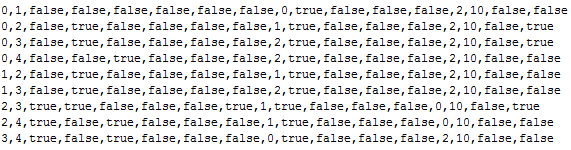
\includegraphics[width=\textwidth]{instance}
\\Các giá trị trong mỗi mẫu của tập huyến luyện cho văn bản trên theo thứ tự là giá trị của các thuộc tính và cuối cùng là loại của mẫu.
\end{block}
\end{frame}

\begin{frame}
\frametitle{Tạo tập huấn luyện và tập kiểm tra}
\begin{block}{}
Cách tạo tập kiểm tra cũng tương tự cách tạo tập huấn luyện ở trên.
\end{block}
\end{frame}

\subsection{Áp dụng giải thuật học máy và đánh giá}
\begin{frame}
\frametitle{Áp dụng giải thuật học máy và đánh giá}
\begin{block}{}
Áp dụng mô hình học có giám sát. Giải thuật cây quyết định J48 (trên Weka) được sử dụng và mô hình được đánh giá bằng các thông số Precision, Recall và F-measure.
\end{block}
\begin{block}{}
Có 2 hướng thực hiện:
\begin{itemize}
\item Sử dụng tập huấn luyện và tập kiểm tra riêng biệt
\item Sử dụng k-fold cross validation (k=10)
\end{itemize}
\end{block}
\end{frame}

\section{Kết quả thực nghiệm}
\begin{frame}
\frametitle{Kết quả thực nghiệm}
\begin{block}{}
Áp dụng mô hình cho dữ liệu gồm 40 review về điện thoại, sử dụng công cụ Weka. Quá trình trích xuất các cụm danh từ và các thuộc tính có sử dụng tới bộ công cụ xử lý ngôn ngữ tự nhiên của Stanford.
\end{block}
\begin{table}[]
\centering
\caption{Các độ đo kết quả}
\label{my-label}
\begin{tabular}{|l|l|l|}
\hline
\textbf{Precision} & \textbf{Recall} & \textbf{F-measure} \\ \hline
0.71               & 0.50            & 0.59               \\ \hline
\end{tabular}
\end{table}
\end{frame}

\section{Tổng kết}
\begin{frame}
\frametitle{Kết luận}

Trong nửa đầu của Luận văn tốt nghiệp, nhóm đã thực hiện được những công việc sau:
\begin{itemize}
\item Tìm hiểu khái quát về bài toán đồng tham chiếu trong XLNNTN và các hướng tiếp cận
\item Tìm hiểu khái quát về khai khoáng ý kiến và các hướng tiếp cận
\item Thực hiện phương pháp đề xuất và cho ra kết quả của mô hình đối với tiếng Anh
\end{itemize}

Trong giai đoạn còn lại, nhiệm vụ của nhóm là:

\begin{itemize}
\item Cải thiện độ chính xác của mô hình cho tiếng Anh bằng cách tối ưu tập thuộc tính
\item Áp dụng một số phương pháp huấn luyện (train) và kiểm tra (test) khác nhằm so sánh và tìm ra phương pháp tốt nhất
\item Thử nghiệm mô hình cho tiếng Việt
\end{itemize}

\end{frame}

\end{document}